\section{Introduction}\label{sec:intro}

\begin{figure*}[t]
  \centering
  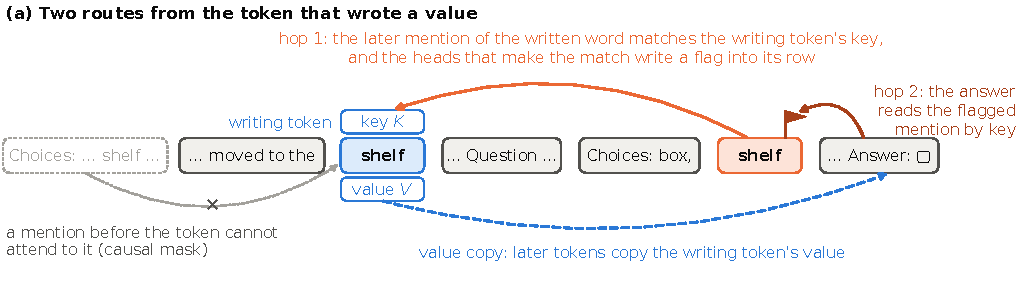
\includegraphics[width=0.87\textwidth]{figures/fig_schematic.pdf}\\[2pt]
  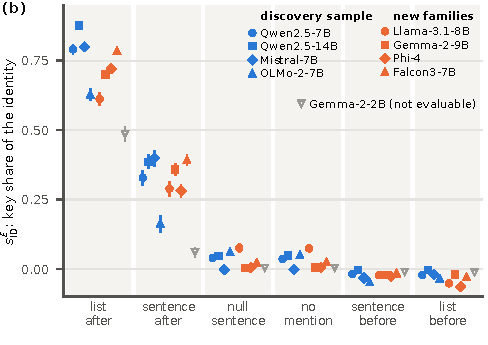
\includegraphics[width=0.49\textwidth]{figures/fig_fresh.pdf}\hfill
  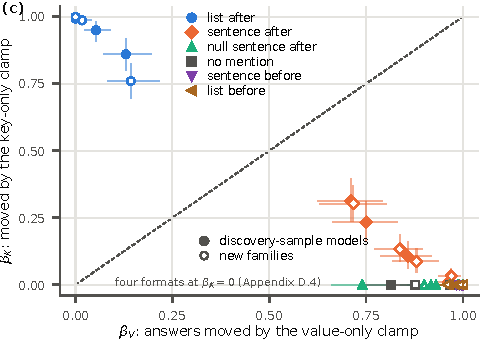
\includegraphics[width=0.49\textwidth]{figures/fig_crossover_main.pdf}
  \caption{\textbf{Later mentions decide whether a written value is looked up through its key or copied from its value.} (a)~The writing token \emph{shelf} leaves a key $K$ and a value $V$ in the cache at every layer, which we clamp separately. (b)~Fresh stories: key share of the identity, $s^{E}_{\mathrm{ID}}$ (E: emitted-form score), by where the candidates are named; 95\,\% two-stage cluster intervals; grey: Gemma-2-2B (n.e.: not evaluable; it failed the competence gate). (c)~Share of generated answers moved to the clamped value by the key-only clamp ($\beta_K$, top) and by the value-only clamp ($\beta_V$, bottom), by format; models, markers and intervals as in (b).}
  \label{fig:schematic}
\end{figure*}

\begin{table*}[t]
  \centering
  \caption{\textbf{What the architecture implies, what known circuits supply, and what we find.} ``Architecture alone'': what QK/OV and the causal mask imply \citep{elhage2021framework}. The last column summarises our estimates; \cref{app:crosswalk,app:stage9} give each cell's verdicts.}
  \label{tab:qkov}
  \scriptsize\setlength{\tabcolsep}{3pt}
  \begin{tabular}{@{}p{0.14\textwidth}p{0.075\textwidth}p{0.245\textwidth}p{0.50\textwidth}@{}}
    \toprule
    Question & Architecture alone & Known circuits & What we find (section) \\
    \midrule
    \raggedright Can a mention \emph{before} the token read its key? & \raggedright No (causal mask) & \raggedright Options before a context cannot attend to it \citep{ok2026lost} & Nor does a later token read the key through it; in the new families a list before even lowers the read slightly below no mention (\S\ref{sec:fresh}) \\
    \raggedright Mentioned after it: looked up or copied? & \raggedright Either; copy route open & \raggedright Duplicate-token and induction heads attend to earlier copies \citep{wang2022ioi,olsson2022context} & Looked up: the key carries most of the identity (eight story, three passage models); copied without a later mention. A neutral sentence opens part of the read, a null sentence almost none, a passage's related-articles sentence little (\S\ref{sec:claim1}) \\
    \raggedright Does the route decide generated answers? & \raggedright Not decided & \raggedright Option-selecting heads \citep{wiegreffe2025answer}, some by query--key alignment \citep{tulchinskii2024wise} & Stories: yes, in all eight models; the sentence read in seven, a small share in most. Passages: with lettered options in all four models; with options named, in most answers in two of three; in free form, answers break into hybrids (\S\ref{sec:claim1}) \\
    \raggedright What does the matching head write, and what sets the sign? & \raggedright Not decided & \raggedright Binding ID vectors \citep{feng2023binding}; an option-routing feature \citep{sun2026persuaded}; S-inhibition \citep{wang2022ioi} & A flag naming no candidate, read by key; it can move the answer, but so do controls, one overlapping it, and removing it leaves about half the key read. The question sets the sign, after hop~1 (exploratory); IOI: key negative, value positive (\S\ref{sec:claim2}) \\
    \raggedright Until when can an edit of the token change the answer? & \raggedright Not decided (every layer's cache is read) & \raggedright Overwriting a field's cached key and value can leave the old decision \citep{bojieli2026notes} & Free form: until most of the depth. Listed after: mainly through early layers, to a model-specific depth; later patches leave the old answer. Single-site steering largely follows this; steering at every position escapes with a named list, mostly not with letters; inside the window the delivered key share predicts transfer to a named list (\S\ref{sec:claim3}) \\
    \bottomrule
  \end{tabular}
\end{table*}

Activation patching, steering vectors and edits of the key--value (KV) cache change a model's state at one context token and read the change in the answer. Whether such an edit reaches the answer at all can depend on where the answer's candidates are named. In three 7--8B models, overwriting the cached key and value of the token that states a value, from a given layer up, changes most free-form answers until \pctn{\NqLcFracNoneMin}--\pct{\NqLcFracNoneMax} of the depth; with the candidates listed after the context, the same overwrite changes fewer than half of them from \pctn{\NqLcFracListedMin}--\pct{\NqLcFracListedMax} of the depth on, and leaves almost all the rest at the old answer, with high probability (\cref{sec:claim3}): an edit validated in free form can decide nothing once the candidates are listed.

The format also changes how the value is read. Mechanistic accounts often credit one cache channel: keys act as routers \citep{ma2025addressbook}, Llama models carry binding information mainly in key vectors \citep{oh2026rebinding}, and refusal steering acts mainly through the OV circuit \citep{cheng2026steering}. Later tokens see a token only through its cached key and value, so a written value can reach the answer in two ways (\cref{fig:schematic}a): it is \emph{looked up} when a later token that already holds a candidate matches the writing token's key, so that the key carries which value was written, and \emph{copied} when the identity travels in the value. We show that where the candidates are mentioned, relative to the token that writes the value, can decide the route, and how deep an edit of that token can act. Whether the accounts above depend on this we did not test (\cref{sec:limitations}).

In the belief stories of \citet{anonymous2026fitted}, one token, which they call the critical token and we call the \emph{writing token}, states where an object was moved. We clamp its cached key and value separately and vary whether and where the candidates are named again: in \nModels{} discovery-sample models from three families; in the final preregistered round (stage 8), on 150 newly drawn stories in eight models from seven families, four never examined before; and on counterfactual reading-comprehension passages. A last experiment (stage 9), in three 7--8B models, overwrites the token's cache from a given layer up or only below it, and writes edits there. The main analyses were fixed before their data were seen (\cref{sec:method}). From \citet{anonymous2026fitted} we take the story template and generator, the prompt encoder and the training recipe of a learned subspace edit (their released edit is revisited in \cref{app:remap}).

\paragraph{What is known, and what we add.}
Known circuits attend to earlier copies, select listed options by query--key alignment and retrieve bound entities (\cref{tab:qkov}; \citealp{tulchinskii2024wise,feng2023binding,dai2024binding,prakash2024finetuning,prakash2025lookbacks,gurarieh2025mixing}), and shallower heads can write a routing feature into option rows \citep{sun2026persuaded}. Without a later mention no later token holds a candidate, so copying is close to forced; with one, both routes are open. We claim no new head type and add three results.
(1)~Where the candidates are mentioned decides the route in every family we tested, and in generated answers: with a later list a value-only clamp changes few of them, and the copy route remains as a fallback (discovery sample; \cref{sec:claim1,sec:claim2}).
(2)~In two 7B models, the heads that make the match (enriched for duplicate-token heads; discovery sample) write at the later mention a component, the \emph{flag}, that is the same whichever value was written, and the answer selects the flagged row by key (a K-composition; \citealp{elhage2021framework}); it can move the answer but is neither specific nor the only carrier (\cref{sec:claim2}).
(3)~With a list after the story, an edit of the writing token acts mainly through its early layers; single-site steering largely follows this window, steering at every position (which also writes at the answer) escapes it with a named list, and inside the window the delivered share of the natural key displacement predicts transfer to a named list. Edits do not keep the model's own key-to-value ratio (\cref{sec:claim3}).
